\chapter{真空能量与德西特视界}

\lectureoverview{真空能量不同于普通物质：它既不选出一个优先的惯性系，也不随宇宙膨胀而稀释。一旦把引力纳入进来，这个表面上无害的能量零点就会改变时空的几何。我们将推导物质主导的规律\(a(t)\propto t^{2/3}\)，将其与真空主导的规律\(a(t)\propto e^{Ht}\)进行对比，然后在共形坐标中重写德西特时空。由此得到的因果图揭示出一个依赖于观测者的、位于固定固有距离处的事件视界。}

\section{真空中的量子涨落}

我们从激发整场讲座的问题开始。量子场论赋予空无一物的空间以能量。这是否意味着真实的电子--正电子对会不断地从虚无中涌现出来？

\begin{classroomqa}
\audiencequestion{电子--正电子对的产生与湮灭真的在真空中发生吗，还是说那只不过是一种记账手段？\lecturetimestamp{00:00:06}}
\lecturerresponse{虚粒子对会对真空能量有所贡献，但它们并不是那种能够被观察到从空无一物的空间中涌现出来的普通粒子。它们是量子基态的涨落，并且只在适合虚过程的限度内持续存在。}
\end{classroomqa}

谐振子给出了最干净的模型。经典地看，它可以静止在其势能的最小值处。量子力学地看，精确地位于最小值处与精确地具有零动量是不相容的。基态在两者之间做出折中，并保留零点能
\begin{equation}
E_0=\frac{1}{2}\hbar\omega.
\label{eq:l08-zero-point}
\end{equation}
这是谐振子所能具有的最低能量。它不是激发态，也不代表一股可观测的粒子流。

自由场分解为简正模，每个模都像一个谐振子那样运动。腔中的电磁场就是一个熟悉的例子。每个模都贡献一个形如式~\eqref{eq:l08-zero-point}中的项；电子、夸克以及其他量子场则贡献它们各自的基态涨落。把这些贡献加起来，就得到我们所谓的真空能量。朴素的微观估计与观测到的宇宙学尺度之间那臭名昭著的不匹配是真实存在的，但它不是本讲的主题。

\begin{classroomqa}
\audiencequestion{大约\(120\)个数量级的差异还会再讨论吗？\lecturetimestamp{00:02:59}}
\lecturerresponse{不在这里讨论。当前的目标是理解宇宙学视界：宇宙学方程如何产生加速膨胀，以及为什么加速膨胀会产生事件视界。}
\end{classroomqa}

\begin{classroomqa}
\audiencequestion{上一讲中的紫外--红外关系是今晚讨论的一部分吗？\lecturetimestamp{00:03:59}}
\lecturerresponse{它以后可能会被重新讨论，但它不是计划中论证的一部分。眼下的路径是从真空能量到宇宙学，然后再到视界。}
\end{classroomqa}

\section{为什么真空能量是洛伦兹不变的}

下一个问题看起来很简单，却揭示出真空能量的定义性属性。如果空无一物的空间具有正的能量密度，为什么它不像光学介质那样起作用并改变光速？

\begin{classroomqa}
\audiencequestion{正的真空能量密度难道不应该产生折射效应，使光传播得稍微慢一些吗？\lecturetimestamp{00:04:35}}
\lecturerresponse{普通物质能够做到这一点，是因为它定义了一个优先的静止系。真空能量则不同：它不选出这样一个系，而且每个惯性观测者都得到相同的真空能量密度。因此对光的局域测量仍然保持不变的速度\(c\)。}
\end{classroomqa}

我们必须把定律的对称性与某个特定状态的对称性区分开来。物理方程可以是平移不变的，尽管斯坦福不是伯克利，地球也不是星际空间。平移\emph{整个}物理安排会使定律保持不变；而物质的实际安排不必在每个位置看起来都一样。同样地，旋转不变的方程并不会使这间教室具有旋转对称性。

同样的区分也适用于洛伦兹变换。气体有一个静止系。穿过它运动的观测者会看到运动的分子和不同的能量密度，因此气体的状态不是洛伦兹不变的，尽管支配它的方程是洛伦兹不变的。普通物质、辐射浴以及实验室装置都通过选出特殊的运动或方向而破坏了这一对称性。

真空能是不这样做的物质的例外形式。设想一个报告真空能密度的探测器。它在静止时给出某个值\(\rho_{\rm vac}\)。加速探测器并重复测量：结果不变。在相对论记号中，这一性质由与度规成正比的应力张量编码，
\begin{equation}
T_{\mu\nu}^{\rm vac}=-\rho_{\rm vac}g_{\mu\nu},
\qquad
p_{\rm vac}=-\rho_{\rm vac}.
\label{eq:l08-vacuum-stress}
\end{equation}
\editorialnote{压强关系并非在黑板上推导出来的。它是讲座中两个定义性质——洛伦兹不变性和膨胀过程中密度恒定——背后的协变陈述。}

局域这一限定很重要。经过观察者的光线用附近的钟和尺测量，其运动速率为\(c\)。在膨胀几何中询问遥远光线相对于我们的速度，需要选择坐标以及比较遥远事件的方案。该坐标速度不必等于\(c\)，尽管每个局域观察者都测得\(c\)。

\begin{classroomqa}
\audiencequestion{在这次讨论中，真空能和宇宙学常数是同义词吗？\lecturetimestamp{00:11:57}}
\lecturerresponse{是的。它们是同一个项在爱因斯坦方程中的两种放置方式：它可以被描述为几何侧的宇宙学常数，或被描述为源侧的洛伦兹不变真空应力能量。}
\end{classroomqa}

\section{什么会稀释，什么不会}

用质量为\(m\)的非相对论性粒子充满一个大区域。在足以对星系和星系团取平均的大尺度上，假设分布是均匀的。如果一个共动体积包含\(N\)个粒子，其物质密度为
\begin{equation}
\rho_m=\frac{Nm}{V}.
\end{equation}
当每个线度加倍时，体积增大\(2^3=8\)，而\(N\)和\(m\)保持不变。因此密度降至其先前值的八分之一。普通物质会稀释，因为同样的粒子占据更大的物理体积。

辐射也会稀释，而且更快。其数密度随体积下降，同时每个光子的波长被拉伸，其能量发生红移。我们稍后将记录结果\(\rho_r\propto a^{-4}\)，但今晚我们不会求解辐射主导的宇宙学。

真空能是例外：
\begin{equation}
\rho_{\rm vac}(t)=\text{constant}.
\label{eq:l08-rho-vac-constant}
\end{equation}
它不会成团，不会选择方向，不会选择惯性系，也不会随着空间膨胀而变得稀薄。如果一个共动盒子增大，其中包含的真空能按体积成比例增大。

\editorialnote{密度恒定并不意味着膨胀的共动盒子内部的总真空能恒定。协变应力能量守恒，
\(\dot\rho+3H(\rho+p)=0\)，之所以得到满足，是因为真空能具有负压强\(p_{\rm vac}=-\rho_{\rm vac}\)。功项恰好提供了盒子总真空能的变化。}

\section{引力看到能量的零点}

在非引力的实验室物理中，将每个能量都移动同一个常数通常不改变任何东西。光谱依赖于差值：激发态原子与未激发原子之间的能量，或者有粒子与无粒子的状态之间的能量。真空似乎不提供任何可以据以测量其绝对能量的参照。

引力改变了问题。质量就是能量，能量产生引力，因此真空能会产生引力。一个在原子跃迁中不可见的常数可以弯曲时空。

爱因斯坦方程将几何与源分开：
\begin{equation}
G_{\mu\nu}=8\pi G_N T_{\mu\nu},
\label{eq:l08-einstein}
\end{equation}
其中单位取\(c=1\)。爱因斯坦张量\(G_{\mu\nu}\)由度规\(g_{\mu\nu}(x)\)及其导数构成。应力张量\(T_{\mu\nu}\)包含来自物质和非引力场的能量密度、动量密度、压强和应力。真空能正如普通物质一样属于这个源侧。\editorialnote{口头介绍简要地将\(8\pi/3\)与张量方程联系起来。因子\(1/3\)属于下面的空间平坦弗里德曼方程，而不属于方程~\eqref{eq:l08-einstein}。}

\begin{figure}[htbp]
\centering
\includegraphics[width=0.62\textwidth]{lecture_08_figure_02.png}
\caption{爱因斯坦方程的几何侧，由时空度规\(g_{\mu\nu}(x)\)构成。}
\lectureframe{00:21:58.820}
\end{figure}

\section{几何被约化为一个标度因子}

我们现在选择具有平坦空间切片的最简单的均匀膨胀几何：
\begin{equation}
ds^2=-dt^2+a(t)^2\,d\mathbf{x}^2,
\qquad
d\mathbf{x}^2=dx^2+dy^2+dz^2.
\label{eq:l08-frw-metric}
\end{equation}
坐标标记\(\mathbf{x}\)被画在一张无限的橡胶片上。它们不必移动，但它们的物理间距会移动。相隔\(\Delta\mathbf{x}\)的两个共动点在固定\(t\)时的固有距离为
\begin{equation}
D(t)=a(t)\lvert\Delta\mathbf{x}\rvert.
\label{eq:l08-proper-distance}
\end{equation}
因此，这个高度对称几何的所有时间依赖性都储存在一个函数中，即标度因子\(a(t)\)。常数\(a\)在空间重标度后给出平坦的闵可夫斯基时空。依赖于时间的\(a\)可以使每个空间切片保持平坦，同时使整个时空弯曲。

\begin{classroomqa}
\audiencequestion{对于坐标标记\(x=7\)和\(x=13\)，它们的坐标间隔是否为\(4\)？\lecturetimestamp{00:27:40}}
\lecturerresponse{不是。它是\(13-7=6\)，因此它们的物理间隔为\(6a(t)\)。这一修正很有用：\(x\)标记共动位置，而乘以\(a(t)\)则给出物理距离。}
\end{classroomqa}

对于该度规和空间均匀的能量密度，爱因斯坦方程的一个分量成为空间平坦的弗里德曼方程，
\begin{equation}
\left(\frac{\dot a}{a}\right)^2
=\frac{8\pi G_N}{3}\rho(t).
\label{eq:l08-friedmann}
\end{equation}
比值
\begin{equation}
H(t)\equiv\frac{\dot a(t)}{a(t)}
\label{eq:l08-hubble-definition}
\end{equation}
即为哈勃参数。在此阶段它是一个定义，并且可以随时间变化。

\begin{figure}[htbp]
\centering
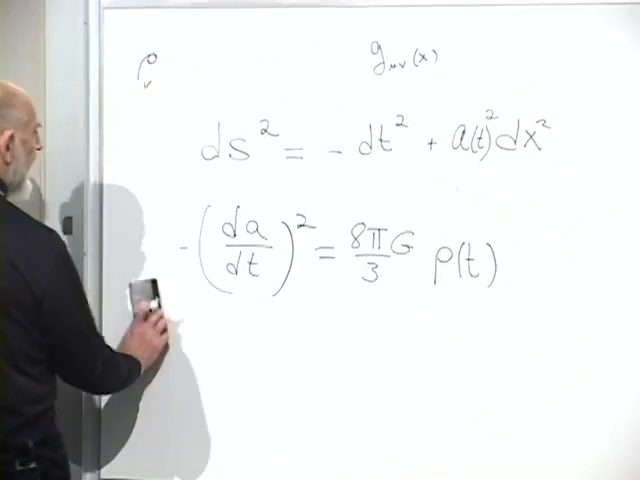
\includegraphics[width=0.90\textwidth]{lecture_08_figure_03.png}
\caption{在板上补回缺失的因子\(1/a^2\)之后的平坦膨胀度规和弗里德曼方程。}
\lectureframe{00:30:30.000}
\end{figure}

\paragraph{能量平衡图像。}
对于这一能量平衡图像，方程~\eqref{eq:l08-friedmann}被示意性地写为
\begin{equation}
-\frac{3}{8\pi G_N}H^2+\rho=0.
\label{eq:l08-energy-heuristic}
\end{equation}
物质能量为正，而由膨胀标度因子代表的引力自由度带有负的动能项。在这个约化问题中，负的引力能加上正的物质量能等于零是一个有用的助记。

\editorialnote{方程~\eqref{eq:l08-energy-heuristic}是高度对称的微超空间模型中的哈密顿约束，而不是一个坐标无关的定理，断言每一个任意宇宙都具有等于零的全局守恒总能量。讲座将其用作对弗里德曼约束的启发式解释。}

\section{物质主导的膨胀}

回到一个共动数学盒子，其坐标边长为\(\Delta x=1\)。它的物理边长为\(a(t)\)，因此其物理体积为\(a(t)^3\)。如果它包含\(N\)个质量为\(m\)的非相对论性粒子，那么
\begin{equation}
\rho_m(t)=\frac{Nm}{a(t)^3}
=\frac{\rho_0}{a(t)^3}.
\label{eq:l08-matter-density}
\end{equation}
粒子本身并不膨胀；膨胀的是它们的平均间距。

\begin{figure}[htbp]
\centering
\includegraphics[width=0.84\textwidth]{lecture_08_figure_04.png}
\caption{在组装共动盒子论证时的度规和弗里德曼方程。}
\lectureframe{00:36:07.940}
\end{figure}

代入方程~\eqref{eq:l08-friedmann}得到
\begin{equation}
\left(\frac{\dot a}{a}\right)^2
=\frac{8\pi G_N\rho_0}{3a^3}.
\end{equation}
记\(K=8\pi G_N\rho_0/3\)并选择膨胀分支：
\begin{align}
\dot a^2&=\frac{K}{a},\\
\dot a&=\sqrt{K}\,a^{-1/2},\\
a^{1/2}\,da&=\sqrt{K}\,dt.
\label{eq:l08-matter-separated}
\end{align}

\begin{classroomqa}
\audiencequestion{分离后的方程应如何求解？\lecturetimestamp{00:38:15}}
\lecturerresponse{对两边积分。\(a^{1/2}\,da\)的积分是\(\frac{2}{3}a^{3/2}\)，而不是\(\frac{3}{2}a^{3/2}\)；\(\frac{3}{2}\)是新的幂次，而\(\frac{2}{3}\)是系数。}
\end{classroomqa}

因此，
\begin{equation}
\frac{2}{3}a^{3/2}
=\sqrt{K}\,(t-t_B),
\end{equation}
其中\(t_B\)是确定所选时间原点的积分常数。除归一化和时间平移外，
\begin{equation}
a(t)\propto (t-t_B)^{2/3}.
\label{eq:l08-matter-solution}
\end{equation}

\begin{figure}[htbp]
\centering
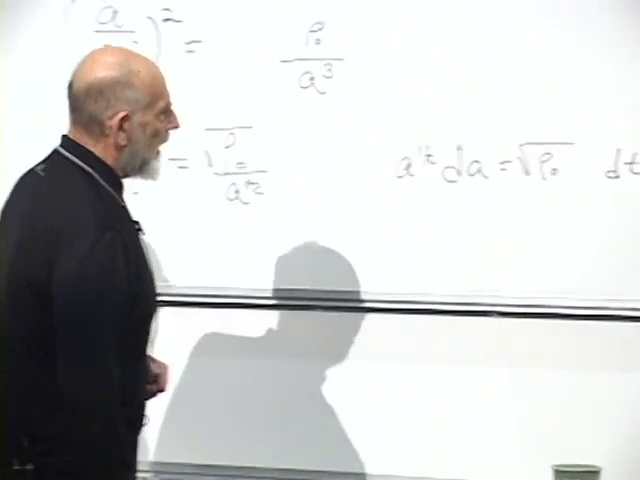
\includegraphics[width=0.86\textwidth]{lecture_08_figure_05.png}
\caption{物质密度代入和变量分离导致\(a^{1/2}da\propto dt\)。}
\lectureframe{00:38:30.000}
\end{figure}

曲线\(t^{2/3}\)比直线增长得更慢。其斜率减小，因此物质主导的宇宙减速。在讲座所用的牛顿语言中，粒子起初彼此分离，而它们之间的相互引力吸引不断降低分离的速率。

\begin{figure}[htbp]
\centering
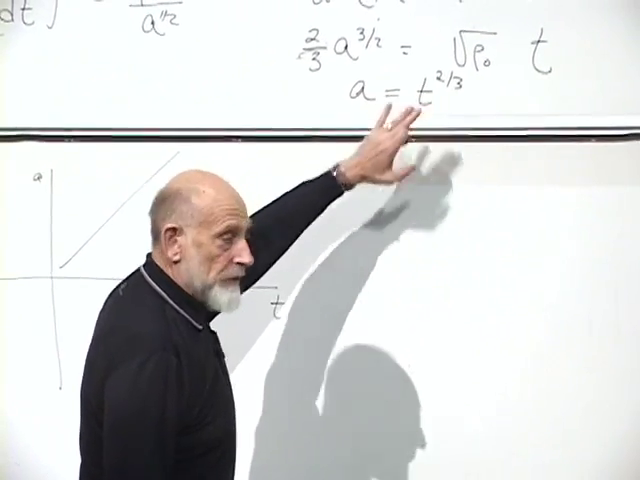
\includegraphics[width=0.86\textwidth]{lecture_08_figure_06.png}
\caption{板上对线性膨胀与向下凹的物质定律\(a(t)\propto t^{2/3}\)的比较。}
\lectureframe{00:40:00.000}
\end{figure}

为了定位，辐射浴有
\begin{equation}
\rho_r\propto a^{-4},
\end{equation}
而不是\(a^{-3}\)：体积稀释贡献三个幂次，宇宙学红移再贡献一个。相应的标度因子也可以求解，但讲座有意将这一练习搁置一旁。

\section{真空主导的膨胀}

现在只在弗里德曼方程右侧放真空能。由于\(\rho_{\rm vac}\)是常数，
\begin{equation}
\left(\frac{\dot a}{a}\right)^2
=\frac{8\pi G_N}{3}\rho_{\rm vac}
\equiv H^2.
\label{eq:l08-de-sitter-friedmann}
\end{equation}
\(H\)有两种用法需要区分开。方程~\eqref{eq:l08-hubble-definition}定义了可能随时间变化的量\(\dot a/a\)。方程~\eqref{eq:l08-de-sitter-friedmann}说明，在纯真空能宇宙中它的值是常数
\begin{equation}
H=\sqrt{\frac{8\pi G_N\rho_{\rm vac}}{3}}.
\end{equation}
取膨胀分支得到
\begin{equation}
\dot a=Ha,
\end{equation}
因此
\begin{equation}
a(t)=C e^{Ht}.
\label{eq:l08-exponential-solution}
\end{equation}
积分常数\(C\)确定共动坐标的任意归一化。正比于\(a\)当前值的增长是指数增长。

\begin{figure}[htbp]
\centering
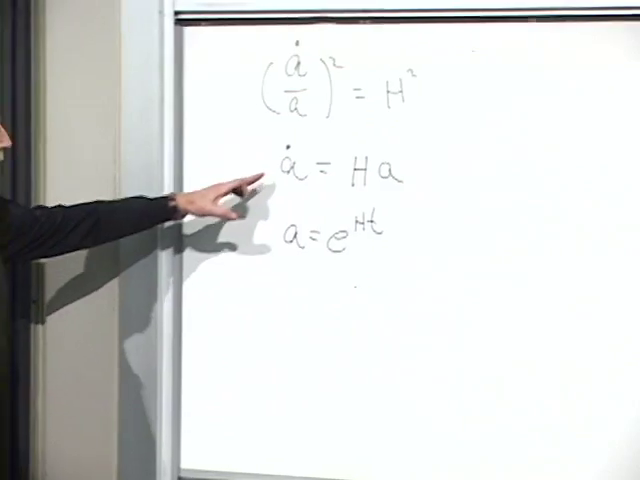
\includegraphics[width=0.88\textwidth]{lecture_08_figure_07.png}
\caption{真空主导的方程\((\dot a/a)^2=H^2\)、它的一阶形式\(\dot a=Ha\)以及指数解。}
\lectureframe{00:47:45.000}
\end{figure}

共动物体的哈勃定律为
\begin{equation}
v_{\rm rec}=HD.
\label{eq:l08-hubble-law}
\end{equation}
在这个纯德西特情形中，退行速率等于\(c\)处的固有距离是常数：
\begin{equation}
D_H=\frac{c}{H},
\label{eq:l08-hubble-radius}
\end{equation}
或在板上所用的\(c=1\)单位下为\(D_H=H^{-1}\)。这个固定尺度将作为德西特事件视界半径在几何上重新出现。\editorialnote{哈勃半径在任意随时间变化的宇宙学中并不自动是事件视界。这一等同在这里成立，是因为在精确德西特空间中\(H\)是常数。}

本讲提出了一个用于真空能探测器的思想实验。将两个极轻的检验物体置于远离其他源的地方，初始时相对于共动流静止，并使它们之间的相互吸引可以忽略。它们的间距遵循指数膨胀。该效应对于地面装置来说实在太小，但宇宙尺度的距离和回溯时间使得同样的物理过程可以被观测到。

\section{从物质主导到真空主导}

本讲所考虑的真实宇宙学模型包含两项：
\begin{equation}
H(t)^2
=\frac{8\pi G_N}{3}
\left(\frac{\rho_0}{a(t)^3}+\rho_{\rm vac}\right).
\label{eq:l08-mixed-friedmann}
\end{equation}
在\(a\)较小时，由于\(a^{-3}\)很大，物质项占主导，解类似于\(t^{2/3}\)。随着宇宙增长，物质被稀释，而真空能保持固定。最终常数项胜出，标度因子向上弯折趋向\(e^{Ht}\)。

\begin{figure}[htbp]
\centering
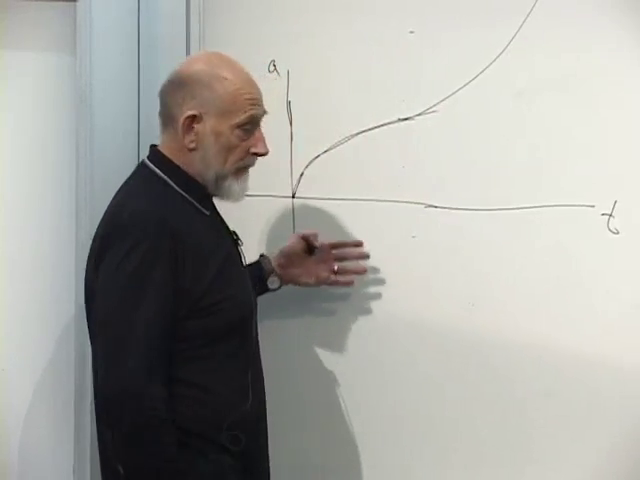
\includegraphics[width=0.87\textwidth]{lecture_08_figure_08.png}
\caption{本讲所描绘的定性转变：早期物质主导的减速，随后是晚期真空主导的指数增长。}
\lectureframe{00:53:30.000}
\end{figure}

\begin{classroomqa}
\audiencequestion{指数解包含一个积分常数。我们怎么知道它不是极其微小？\lecturetimestamp{00:52:41}}
\lecturerresponse{我们测量它。向宇宙更远处看意味着向更早的过去看，因此不同距离上的观测重建的是膨胀曲线较早的部分，而不仅仅是它今天的值。}
\end{classroomqa}

本讲报告说，当时可获得的晚期观测在约百分之五的水平上与指数分支一致，并将这些证据描述为令人信服的，尽管不如电子性质那样的精密测量那样精确。这应被理解为本讲的历史评估，而非当今的精密陈述。

\begin{classroomqa}
\audiencequestion{向上弯折的膨胀曲线最终是否会阻止我们将观测追溯到宇宙大爆炸或宇宙微波背景？\lecturetimestamp{00:55:05}}
\lecturerresponse{这不是作为外推图形的问题来探讨的。相关的、不变量意义上的问题是事件视界的存在性，而这正是我们现在转向的因果问题。}
\end{classroomqa}

\section{束缚系统与遥远未来}

如果指数膨胀持续下去，每一个被稀释的成分与\(\rho_{\rm vac}\)相比都变得可以忽略。这并不意味着原子、太阳系或星系本身被拉伸开来。被束缚得足够强而保持束缚的系统不遵循哈勃流。

\begin{classroomqa}
\audiencequestion{今天没有在膨胀的星系，当真空能占主导时最终会膨胀吗？\lecturetimestamp{00:57:44}}
\lecturerresponse{束缚系统保持束缚。银河系和仙女座星系属于将保持在一起的近邻结构，而已经随膨胀运动的足够遥远的星系继续向外运动，最终越过我们的视界。}
\end{classroomqa}

\emph{被吸引}与\emph{被束缚}之间的区分至关重要。以超过逃逸速度发射的火箭仍然处于地球的吸引引力之下，然而它不会返回。同样，普通引力吸引可能是两个星系之间最大的局域力，而它们的相对轨道却未必是束缚的。

\begin{classroomqa}
\audiencequestion{我们的星系在引力上与一个星系群相关联。加速膨胀最终会克服那种吸引吗？\lecturetimestamp{00:59:17}}
\lecturerresponse{只有局域结构中真正束缚的部分会保持在一起。作为一个描述性标签的星系团是不够的；束缚意味着相对运动低于逃逸。更遥远的星系可以被吸引，却仍然以超过逃逸速度退行。}
\end{classroomqa}

为了直观理解，本讲将相对径向加速度示意性地表示为一个吸引的平方反比项加上一个与间距成正比的真空项：
\enlargethispage{2pt}
\begin{equation}
\ddot r\sim-\frac{G_NM}{r^2}+H^2r.
\label{eq:l08-newtonian-vacuum}
\end{equation}
在理想化的德西特极限下，这些系数与时间无关。第二项之所以增长，仅仅是因为\(r\)增长；它并非源于\(G_N\)的逐渐减弱。

\editorialnote{方程~\eqref{eq:l08-newtonian-vacuum}是一个牛顿式的相对加速度启发式表述，而不是广义相对论中额外的基本力定律。在精确的德西特空间中，相邻的自由下落世界线的相对加速度正比于\(H^2r\)。}

\begin{figure}[htbp]
\centering
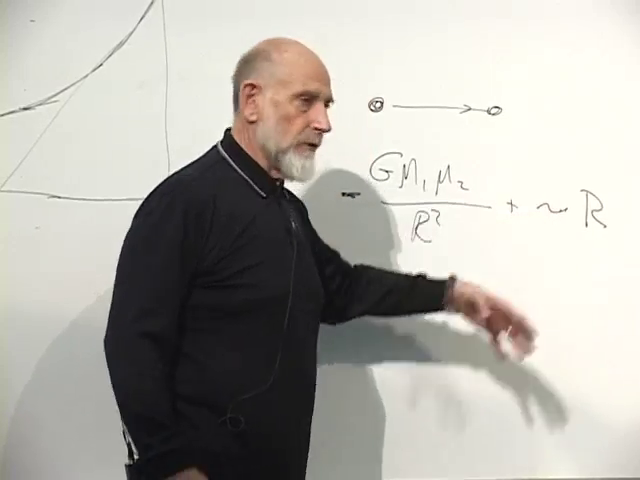
\includegraphics[width=0.88\textwidth]{lecture_08_figure_09.png}
\caption{黑板上对平方反比吸引与随间距线性增长的有效真空排斥之间的比较。}
\lectureframe{01:04:10.000}
\end{figure}

\begin{classroomqa}
\audiencequestion{向外的效应本身会随时间增大吗？\lecturetimestamp{01:01:18}}
\lecturerresponse{在固定间距下不会。其系数是常数。自由退行的物体彼此越来越远，于是正比于\(r\)的项因距离更大而更大。}
\end{classroomqa}

\begin{classroomqa}
\audiencequestion{能否把净效应描述为牛顿常数逐渐减小？\lecturetimestamp{01:02:30}}
\lecturerresponse{不能。\(G_N\)保持常数。在指定间距下，两个系数都不变；随距离改变的只是\(1/r^2\)吸引与正比于\(r\)的项之间的相对重要性。}
\end{classroomqa}

\begin{classroomqa}
\audiencequestion{在真空能变得重要之前的早期宇宙中，同样的星系是否受引力束缚？\lecturetimestamp{01:05:03}}
\lecturerresponse{普通吸引占主导本身并不蕴含束缚。许多星系当时已经在以逃逸速率或更高的速率彼此分离。真空能后来决定大尺度膨胀是减速趋向再坍缩还是加速远离，但最大力与束缚轨道仍是不同的陈述。}
\end{classroomqa}

因此，遥远未来的观测者可能生活在一个已经并合的局部结构中，而每一个未束缚的星系都已变得不可观测。若没有历史记录，该观测者可以有理由地推断宇宙几乎空无一物。这种因果上的孤独，而非局部物体的毁灭，才是通向视界的物理前导。

\section{事件视界的含义}

在破缺之后，令
\begin{equation}
a(t)=e^{Ht}
\end{equation}
并将度规写为
\begin{equation}
ds^2=-dt^2+e^{2Ht}d\mathbf{x}^2.
\label{eq:l08-de-sitter-metric}
\end{equation}

\begin{classroomqa}
\audiencequestion{这个度规所描述的时空叫什么名字？\lecturetimestamp{01:08:13}}
\lecturerresponse{它是德西特时空，通常简称为德西特空间。其视界之所以重要，是因为真空主导的宇宙在晚期趋近于这一几何。}
\end{classroomqa}

在画出其因果结构之前，先回顾彭罗斯图的作用。无穷区间被压缩到一幅有限的图中，而零射线仍保持在\(45^\circ\)。在平直时空中，有质量物体终止于未来类时无穷，零射线终止于零无穷，而一个被允许任意长久等待的惯性观测者没有事件视界排除某个永久的时空区域。

\begin{figure}[htbp]
\centering
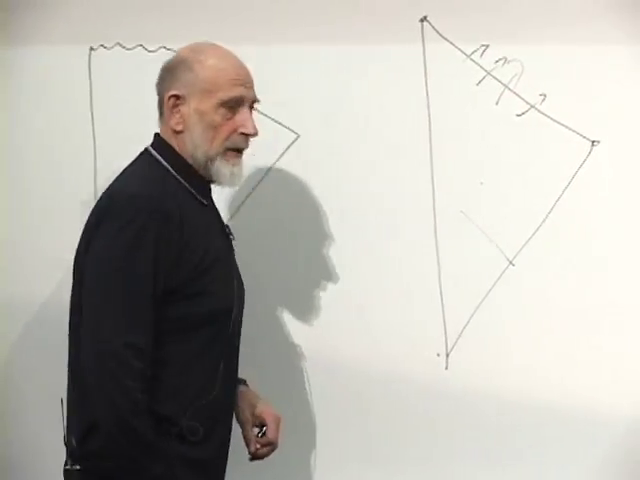
\includegraphics[width=0.80\textwidth]{lecture_08_figure_10.png}
\caption{在引入视界之前，用来区分类时与零终点的平直时空彭罗斯图。}
\lectureframe{01:10:35.000}
\end{figure}

黑洞图提供了对照。外部观测者只能接收来自该观测者未来世界线因果过去的信号。即使观测时间趋于无穷，内部区域仍被排除。能与该观测者通信的事件与永远不能通信的事件之间的边界，就是事件视界。

\begin{definition}
观测者的事件视界是那些事件所成集合的边界：从这些事件出发，未来指向的因果信号能够到达该观测者的世界线。
\label{def:l08-event-horizon}
\end{definition}

\begin{figure}[htbp]
\centering
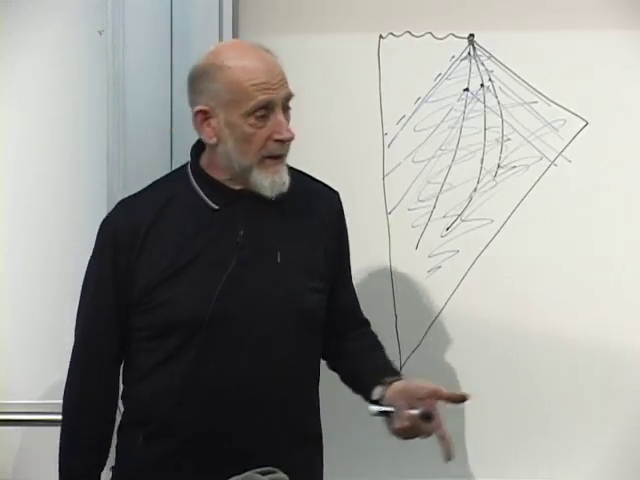
\includegraphics[width=0.80\textwidth]{lecture_08_figure_11.png}
\caption{与黑洞的对照：来自任意晚的外部观测的后向光锥永远不包含事件视界之外的区域。}
\lectureframe{01:13:50.000}
\end{figure}

因此，事件视界是一个全局因果边界，而不仅仅是某个物体今天恰好看起来暗淡的距离。要确定它的位置，必须知道即使经过任意长久的等待，哪些信号仍能到达。

\section{压缩无穷未来}

方程~\eqref{eq:l08-de-sitter-metric}中的空间坐标已经覆盖一个无穷平直切片。我们将不动它们，只压缩时间。引入共形时间\(T\)，要求
\begin{equation}
dt^2=e^{2Ht}dT^2.
\label{eq:l08-conformal-definition}
\end{equation}
取未来指向的平方根并整理，得到
\begin{equation}
dT=e^{-Ht}dt.
\end{equation}

\begin{classroomqa}
\audiencequestion{这个积分是什么，包括其符号？\lecturetimestamp{01:17:25}}
\lecturerresponse{它是\(-H^{-1}e^{-Ht}\)。一个加性常数只是平移\(T\)的原点，因此选择它使无穷未来位于\(T=0\)。}
\end{classroomqa}

因此
\begin{equation}
T=-\frac{1}{H}e^{-Ht},
\qquad -\infty<T<0.
\label{eq:l08-conformal-time}
\end{equation}
当\(t\to-\infty\)时，\(T\to-\infty\)。当固有时\(t\to+\infty\)时，\(T\to0^{-}\)。无穷未来已被置于有限的水平线\(T=0\)上；没有观测者在有限固有时内到达它。

\begin{figure}[htbp]
\centering
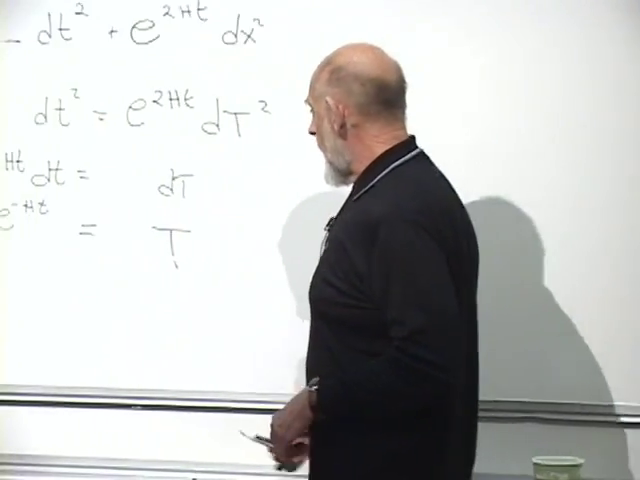
\includegraphics[width=0.86\textwidth]{lecture_08_figure_12.png}
\caption{共形时间积分以及无穷未来\(t\to+\infty\)到\(T=0^{-}\)的映射。}
\lectureframe{01:19:10.000}
\end{figure}

由方程~\eqref{eq:l08-conformal-time}，
\begin{equation}
HT=-e^{-Ht},
\qquad
e^{2Ht}=\frac{1}{H^2T^2}.
\label{eq:l08-conformal-factor}
\end{equation}
将\(dt=e^{Ht}dT\)用于方程~\eqref{eq:l08-de-sitter-metric}，便得到
\begin{equation}
ds^2=\frac{1}{H^2T^2}
\left(-dT^2+d\mathbf{x}^2\right).
\label{eq:l08-conformal-metric}
\end{equation}
括号中的表达式是闵可夫斯基度规。现在，全部德西特几何都位于一个共同的共形因子中，该因子在\(T\to0^{-}\)时发散。

\begin{figure}[htbp]
\centering
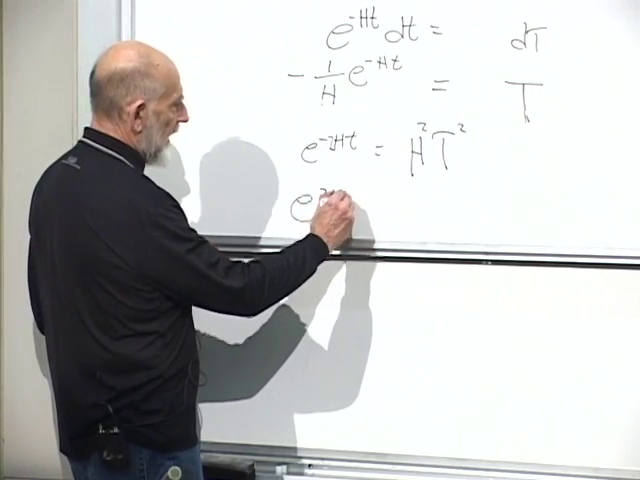
\includegraphics[width=0.87\textwidth]{lecture_08_figure_13.png}
\caption{将\(e^{2Ht}\)与\(1/(H^2T^2)\)联系起来的代数，为度规的共形形式作准备。}
\lectureframe{01:22:50.000}
\end{figure}

\begin{classroomqa}
\audiencequestion{在这个度规中，什么条件决定了光线的路径？\lecturetimestamp{01:23:49}}
\lecturerresponse{光线沿零路径传播，\(ds^2=0\)。因此共同的共形因子相消，沿选定的空间方向留下\(dT=\pm dx\)。}
\end{classroomqa}

在\((T,x)\)图中，光线是\(45^\circ\)的直线：
\begin{equation}
\frac{dx}{dT}=\pm1.
\label{eq:l08-null-lines}
\end{equation}
坐标图在\(T=0\)附近被高度压缩，但它恰好保留了我们需要的信息：哪些事件能够通信。

\begin{figure}[htbp]
\centering
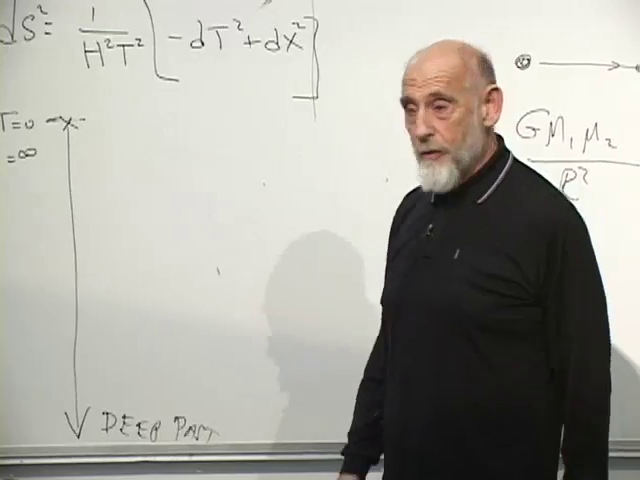
\includegraphics[width=0.86\textwidth]{lecture_08_figure_14.png}
\caption{在用到零条件\(ds^2=0\)以恢复\(45^\circ\)光线的那一刻的共形度规。}
\lectureframe{01:24:05.000}
\end{figure}

\section{德西特空间中的Alice与Bob}

将Alice置于固定的共动位置\(x=0\)。她的世界线竖直上升，并在图中终止于\(T=0\)，尽管她的手表需要无限长的固有时才能到达那里。从该端点画出指向过去的零射线。它们界定了Alice能够接收到信号的极大区域。其外的事件永远不可及。

\begin{figure}[htbp]
\centering
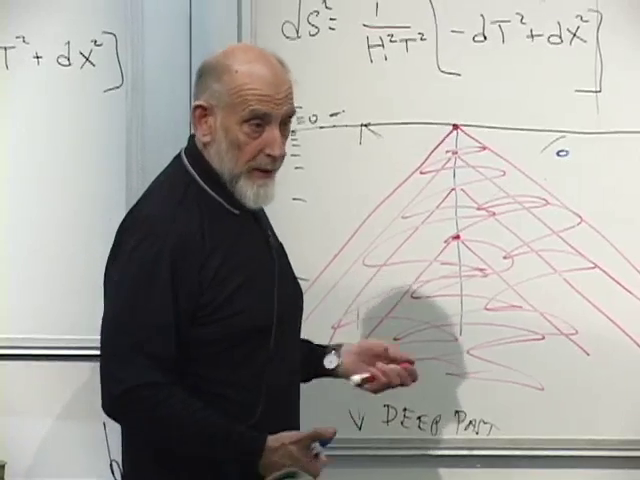
\includegraphics[width=0.88\textwidth]{lecture_08_figure_15.png}
\caption{Alice的极限过去光锥。其零边界是她依赖于观测者的德西特事件视界。}
\lectureframe{01:28:50.000}
\end{figure}

这个视界是私有的。不同的观测者有不同的未来端点，因而有不同的极限过去光锥。假设Bob曾经位于Alice的因果区域内，且两人交换过信息。如果Bob后来随哈勃流穿过Alice的视界，那么穿越之后发出的信号无法到达Alice，无论她等待多久。Bob有自己的视界，并最终失去接收Alice晚期信号的相应能力。

\begin{figure}[htbp]
\centering
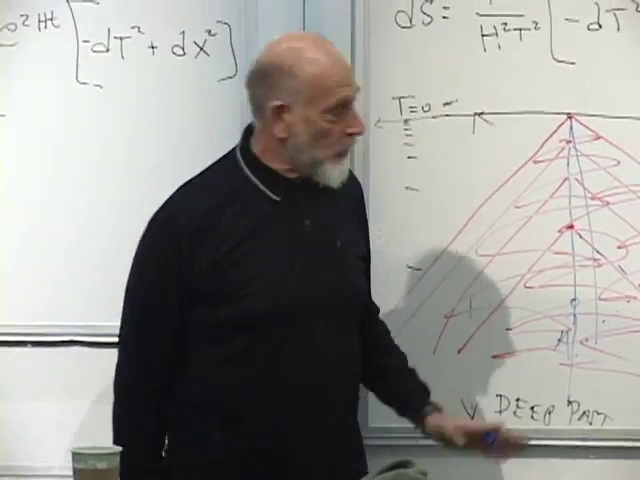
\includegraphics[width=0.88\textwidth]{lecture_08_figure_16.png}
\caption{Alice与Bob各有不同的因果边界。共动的Bob可以离开Alice的因果过去，尽管他们此前交换过信号。}
\lectureframe{01:30:20.000}
\end{figure}

如果Alice和Bob手拉手，或者更现实地说，保持在固定的固有间隔上束缚在一起，那么随着\(a^{-1}\)，他们的共动坐标间隔会缩小。在共形图中他们的曲线彼此靠近，但这并不意味着他们的固有距离消失。增长的共形因子补偿了缩小的坐标间隔，通信可以无限期地保持可能。

\begin{classroomqa}
\audiencequestion{在视界将他们分隔之后，Bob能同时看到Alice吗？\lecturetimestamp{01:31:43}}
\lecturerresponse{没有任何观测者会以那种字面意义同时看到一个遥远事件；观测总是对过去光锥中某个事件的观测。更准确的说法是，在穿越视界之后，来自另一条世界线的新发出的信号都无法到达。}
\end{classroomqa}

在远期宇宙学应用中，Alice代表我们束缚的局域残余，Bob代表每个未束缚的遥远星系。这些星系并不会在Alice时钟的某个有限时刻突然熄灭。它们后来的信号被拉伸到更长的时间间隔，并红移到更长的波长，直到在物理上变得不可探测。

\begin{classroomqa}
\audiencequestion{理论真的说在远期未来不会再有遥远的星系可见吗？\lecturetimestamp{01:33:38}}
\lecturerresponse{未束缚的星系越过局域观测者的事件视界。它们最后可见的信号变得越来越延迟、越来越红移，实际上只留下束缚的局域结构可观测。}
\end{classroomqa}

\section{视界处的红移}

仍然可以画出Bob发出的一个古老光信号在很晚的共形时刻到达Alice，这会使她看起来仍在看到他。物理内容在于这些信号的间隔和能量。Bob时钟的相等间隔到达时，被Alice固有时中越来越大的间隔所分隔。频率和光子能量下降：
\begin{equation}
\nu_{\rm received}\longrightarrow0,
\qquad
E_{\rm received}=h\nu_{\rm received}\longrightarrow0.
\end{equation}
Bob的影像变慢、变红并逐渐消失。极限信号携带的可利用信息趋于零。

\begin{figure}[htbp]
\centering
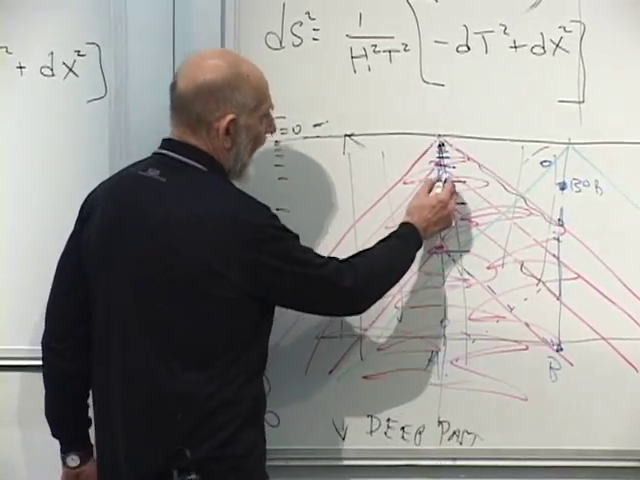
\includegraphics[width=0.89\textwidth]{lecture_08_figure_17.png}
\caption{比较德西特视界红移与熟悉的黑洞视界外部图像的后期板书状态。}
\lectureframe{01:36:20.000}
\end{figure}

\begin{classroomqa}
\audiencequestion{这像黑洞吗？在黑洞情形中，外部观测者永远看不到下落物体穿过视界。\lecturetimestamp{01:36:09}}
\lecturerresponse{是的。在两种情形中，观测者接收到的信号都越来越红移，并且从未直接看到穿越完成。因果图说明了哪些后来的发射永远无法到达；红移则解释了最后可观测的信息如何逐渐消失。}
\end{classroomqa}

这个类比引出了关于温度的问题。

\begin{classroomqa}
\audiencequestion{Alice如何能测量视界正上方的温度？\lecturetimestamp{01:39:34}}
\lecturerresponse{从操作上讲，她可以把温度计系在缆绳上放下去，使其不越过视界，然后再收回来。de Sitter观测者可以想象在宇宙学视界附近进行类似的实验。在量子理论中视界是热的，但本次讲座止步于经典几何，将那个计算推迟。}
\end{classroomqa}

这里没有推导de Sitter温度的公式。Hawking辐射只是作为对这一经典图像的量子修正的预告而出现。

\section{固定的视界半径}

共形图可以翻译回原来的时间坐标。两个共动点保持固定的坐标间隔，满足
\begin{equation}
D(t)=e^{Ht}\lvert\Delta x\rvert,
\end{equation}
因此它们的固有距离按指数增长。

\begin{classroomqa}
\audiencequestion{同样的运动在原来的、未变换的时间坐标中看起来是什么样子？\lecturetimestamp{01:41:14}}
\lecturerresponse{对于固定的共动坐标，整个空间度规随\(e^{2Ht}\)增长；因此固有间隔按\(e^{Ht}\)增长。撤销坐标变换就使这一膨胀变得明确。}
\end{classroomqa}

视界的行为不同，因为它与Alice之间的共动坐标距离并不固定。从终止于\(T=0\)的\(45^\circ\)零测地线来看，在恒定\(T<0\)的切片上视界距离为
\begin{equation}
\Delta x_H=-T=\frac{1}{H}e^{-Ht}.
\label{eq:l08-coordinate-horizon}
\end{equation}
乘以尺度因子得到
\begin{equation}
D_H(t)=a(t)\Delta x_H
=e^{Ht}\frac{e^{-Ht}}{H}
=\frac{1}{H}.
\label{eq:l08-fixed-horizon}
\end{equation}
恢复单位后，\(D_H=c/H\)。坐标间隔缩小，度规尺度增长，而它们的乘积保持不变。

\begin{classroomqa}
\audiencequestion{随着时间推移，从Alice到视界的距离是增长、缩小还是保持不变？\lecturetimestamp{01:42:42}}
\lecturerresponse{它保持不变。其坐标距离缩小，而共形因子增长，使得固有视界半径在\(c=1\)的单位下固定为\(H^{-1}\)。}
\end{classroomqa}

\begin{figure}[H]
\centering
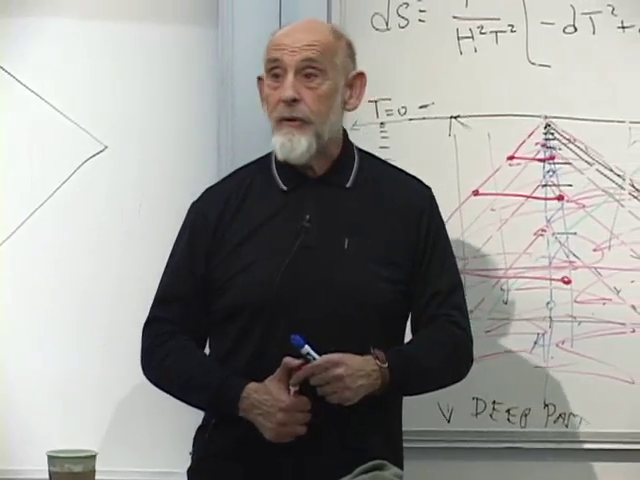
\includegraphics[width=0.90\textwidth]{lecture_08_figure_18.png}
\caption{最终的板书状态：相继的水平切片到视界的坐标距离不断缩小，但固有距离相同。}
\lectureframe{01:43:20.000}
\end{figure}

\begin{classroomqa}
\audiencequestion{Alice是否因为旧的图像从未完全消失而继续看到过去投影到视界上？\lecturetimestamp{01:43:45}}
\lecturerresponse{在经典上，这些图像只在极限意义上持续存在，即它们因无界红移而变得越来越难以探测。这一陈述忽略了与视界相关的Hawking辐射，它将修正量子描述。}
\end{classroomqa}

因此讲座在一个精确的边界处结束。真空能产生了指数膨胀；指数膨胀产生了一个固定的、依赖于观测者的事件视界；而该视界附近的信号已被驱动到趋于零的频率。视界的温度和Hawking辐射属于接下来的内容。正如Susskind所说，假设我们不会越过彼此的视界，我们将在下一讲再见。
